\label{Julian}

Der 'Creator' wurde dazu entwickelt, um dem Benutzer die Möglichkeit zu geben, einen Self-Assesment-Test zu erstellen ohne die dafür anderweitig nötigen Programmierkenntnisse zu besitzen.
Das Programm verfügt über weitreichende Funktionen, damit ein vollständiger Test erstellt werden kann. 
In diesem Abschnitt werden diese Funktionen erläutert und eine Gesamtübersicht über diese Komponente gegeben. 

\subsubsection{Übersicht}
\begin{figure*}[htbp] 
  \centering
     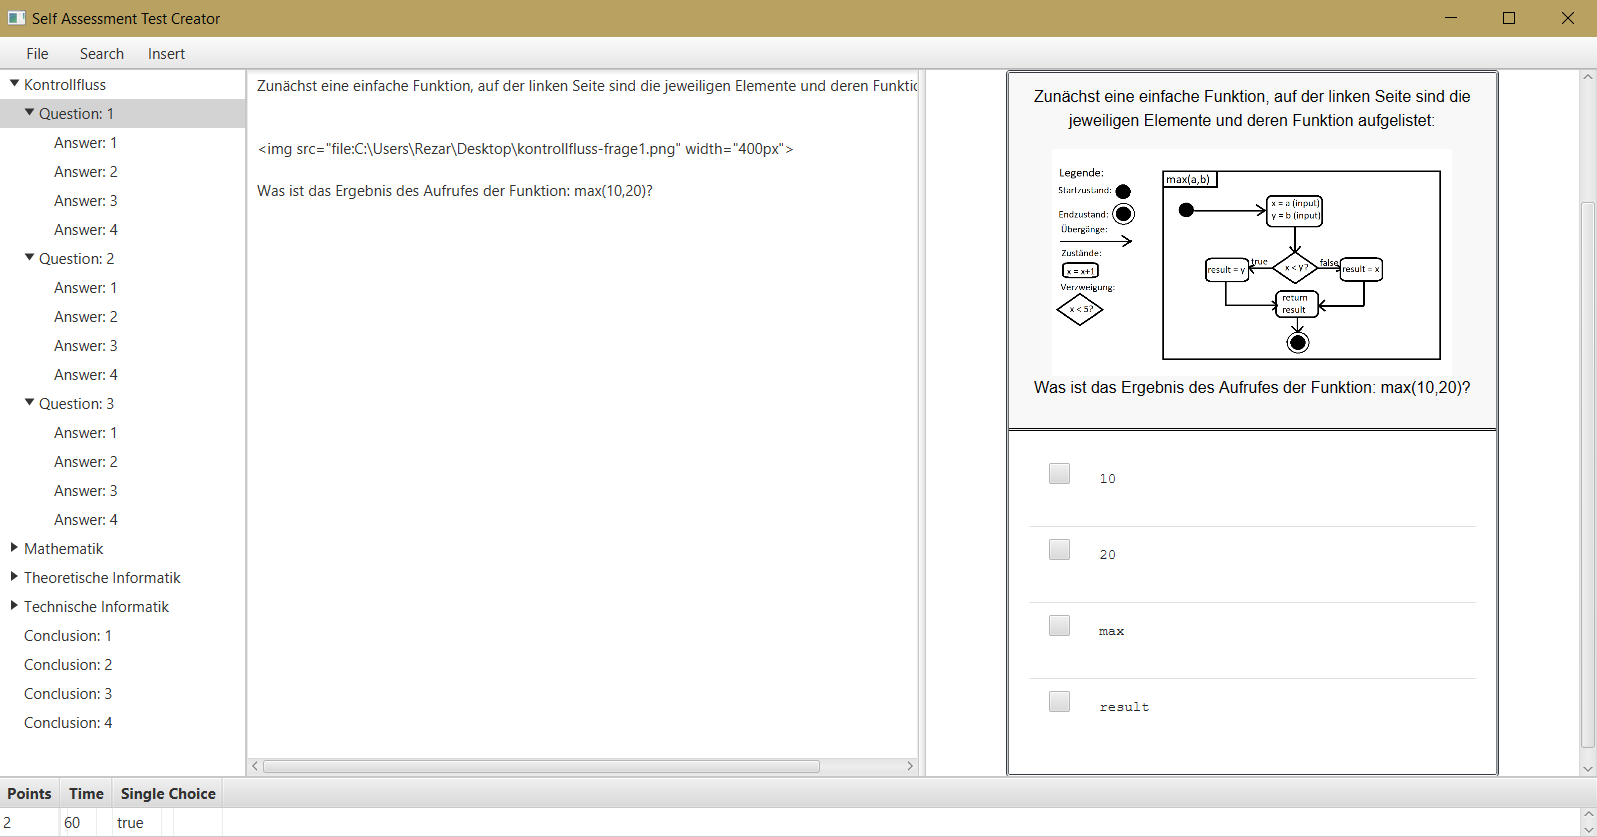
\includegraphics[width=\textwidth]{Julian_Images/Creator-Uebersicht.png}
  \caption{}
  \label{fig:Bild0}
\end{figure*}
Das Hauptfenster des 'Creators', zu sehen in Abbildung~\ref{fig:Bild0}, beinhaltet fünf wichtige Elemente die zur Übersicht und Erstellung des Tests dienen.
Auf der linken Seite ist ein 'TreeView'(A), der die Struktur des Testes darstellt.
In ihm werden die Kategorien, deren zugehörigen Fragen, Antworten und die Feedbacks angezeigt.
In jedem 'TreeItem' wird der Bezeichner des jeweiligen Objekts angezeigt.

Im Zentrum gibt es ein großes Textfeld (B), das den Inhalt des momentan ausgewählten 'TreeItems' wiedergibt.
Im Textfeld kann dieser Inhalt mithilfe von HTML und Markdown editiert werden.

Im unteren Bereich (C) wird eine Tabelle erstellt, die alle Attribute des im 'TreeView'  ausgewählten Elements anzeigt.
Kategorien besitzen als Attribut ihren Namen.
Fragen hingegen haben die Attribute Punkte und Zeit.
Verschiedenen Feebacks können hier verschiedene Punktebereiche zugeordnet werden.

Die obere Leiste (D) enthält 'MenuItems' mit mehreren Funktionen, die im nächsten Abschnitt näher betrachtet werden.

Auf der rechten Seite gibt es ein großes Vorschaufenster (E). 
Dieses zeigt eine Vorschau der gerade ausgewählten Frage an.


\subsubsection{Funktionen}
Unter der Option 'File' gibt es neun Buttons, die nach Funktionen sortiert sind. 
Die ersten vier, also 'New Category', 'New Question', 'New Answer' und 'New Conclusion', erstellen die jeweils zugehörigen Objekte.
'Delete Item' entfernt ein ausgewähltes Objekt.
Generate Website' erstellt einen Zip-Ordner, der die fertige Webseite enthält.
Mit 'Import XML' und 'Export XML' kann der Ersteller den bisherigen Forschritt in einer XML-Datei speichern, beziehungsweise einen bereits erstellten Test laden.
Das letzte 'MenuItem' 'Exit'  beendet das Programm.

Die zweite Option 'Insert' ist dazu da, Medien in Form von Bildern oder Videos in das Textfeld einzufügen. 
Dabei wird ein Medium eingefügt, indem der Ersteller den zugehörigen Dateinamen angibt.
 
